\documentclass[12pt]{article}

%%%%%%%%%%%%%%%%%%%%%%%%%%%%%%%%%%%%%%%%%%%%%%%%%%%%%%%%%%%%%%%%%%%%%%%%%%%%%%%%
%                           Package preset for homework
%%%%%%%%%%%%%%%%%%%%%%%%%%%%%%%%%%%%%%%%%%%%%%%%%%%%%%%%%%%%%%%%%%%%%%%%%%%%%%%%
% Miscellaneous
\usepackage[margin=1in]{geometry}
\usepackage[utf8]{inputenc}
\usepackage{indentfirst}
\usepackage{blindtext}
\usepackage{graphicx}
\usepackage{xr-hyper}
\usepackage{hyperref}
\usepackage{enumitem}
\usepackage{color}
\usepackage{float}
% Math
\usepackage{latexsym}
\usepackage{amsfonts}
\usepackage{amssymb}
\usepackage{amsmath}
\usepackage{commath}
\usepackage{amsthm}
\usepackage{bbold}
\usepackage{bm}
% Physics
\usepackage{physics}
\usepackage{siunitx}
% Code typesetting
\usepackage{listings}
% Citation
\usepackage[authoryear]{natbib}
\usepackage{appendix}
\usepackage[capitalize]{cleveref}
% Title & name
\title{Homework}
\author{Tien Vo}
\date{\today}


%%%%%%%%%%%%%%%%%%%%%%%%%%%%%%%%%%%%%%%%%%%%%%%%%%%%%%%%%%%%%%%%%%%%%%%%%%%%%%%%
%                   User-defined commands and environments
%%%%%%%%%%%%%%%%%%%%%%%%%%%%%%%%%%%%%%%%%%%%%%%%%%%%%%%%%%%%%%%%%%%%%%%%%%%%%%%%
%%% Misc
\sisetup{load-configurations=abbreviations}
\newcommand{\due}[1]{\date{Due: #1}}
\newcommand{\hint}{\textit{Hint}}
\let\oldt\t
\renewcommand{\t}[1]{\text{#1}}

%%% Bold sets & abbrv
\newcommand{\N}{\mathbb{N}}
\newcommand{\Z}{\mathbb{Z}}
\newcommand{\R}{\mathbb{R}}
\newcommand{\Q}{\mathbb{Q}}
\let\oldP\P
\renewcommand{\P}{\mathbb{P}}
\newcommand{\LL}{\mathcal{L}}
\newcommand{\FF}{\mathcal{F}}
\newcommand{\HH}{\mathcal{H}}
\newcommand{\NN}{\mathcal{N}}
\newcommand{\ZZ}{\mathcal{Z}}
\newcommand{\RN}[1]{\textup{\uppercase\expandafter{\romannumeral#1}}}
\newcommand{\ua}{\uparrow}
\newcommand{\da}{\downarrow}

%%% Unit vectors
\newcommand{\xhat}{\vb{\hat{x}}}
\newcommand{\yhat}{\vb{\hat{y}}}
\newcommand{\zhat}{\vb{\hat{z}}}
\newcommand{\nhat}{\vb{\hat{n}}}
\newcommand{\rhat}{\vb{\hat{r}}}
\newcommand{\phihat}{\bm{\hat{\phi}}}
\newcommand{\thetahat}{\bm{\hat{\theta}}}

%%% Other math stuff
\providecommand{\units}[1]{\,\ensuremath{\mathrm{#1}}\xspace}
% Set new style for problem
\newtheoremstyle{problemstyle}  % <name>
        {10pt}                   % <space above>
        {10pt}                   % <space below>
        {\normalfont}           % <body font>
        {}                      % <indent amount}
        {\bfseries\itshape}     % <theorem head font>
        {\normalfont\bfseries:} % <punctuation after theorem head>
        {.5em}                  % <space after theorem head>
        {}                      % <theorem head spec (can be left empty, 
                                % meaning `normal')>

% Set problem environment
\theoremstyle{problemstyle}
\newtheorem{problemenv}{Problem}[section]
\newenvironment{problem}[1]{%
  \renewcommand\theproblemenv{#1}%
  \problemenv
}{\endproblemenv}
% Set lemma environment
\newenvironment{lemma}[2][Lemma]{\begin{trivlist}
\item[\hskip \labelsep {\bfseries #1}\hskip \labelsep {\bfseries #2.}]}{\end{trivlist}}
% Set solution environment
\newenvironment{solution}{
    \begin{proof}[Solution]$ $\par\nobreak\ignorespaces
}{\end{proof}}
\numberwithin{equation}{problemenv}

%%% Page format
\setlength{\parindent}{0.5cm}
\setlength{\oddsidemargin}{0in}
\setlength{\textwidth}{6.5in}
\setlength{\textheight}{8.8in}
\setlength{\topmargin}{0in}
\setlength{\headheight}{18pt}

%%% Code environments
\definecolor{dkgreen}{rgb}{0,0.6,0}
\definecolor{gray}{rgb}{0.5,0.5,0.5}
\definecolor{mauve}{rgb}{0.58,0,0.82}
\lstset{frame=tb,
  language=Python,
  aboveskip=3mm,
  belowskip=3mm,
  showstringspaces=false,
  columns=flexible,
  basicstyle={\small\ttfamily},
  numbers=none,
  numberstyle=\tiny\color{gray},
  keywordstyle=\color{blue},
  commentstyle=\color{dkgreen},
  stringstyle=\color{mauve},
  breaklines=true,
  breakatwhitespace=true,
  tabsize=4
}
\lstset{
  language=Mathematica,
  numbers=left,
  numberstyle=\tiny\color{gray},
  numbersep=5pt,
  breaklines=true,
  captionpos={t},
  frame={lines},
  rulecolor=\color{black},
  framerule=0.5pt,
  columns=flexible,
  tabsize=2
}


\title{Homework 10: Phys 7320 (Spring 2022)}
\due{April 6, 2022}

\begin{document}
\maketitle
%%%%%%%%%%%%%%%%%%%%%%%%%%%%%%%%%%%%%%%%%%%%%%%%%%%%%%%%%%%%%%%%%%%%%%%%%%%%%%%
\begin{problem}{10.1}[The electric field of a relativistic particle]
In class we showed that the Faraday tensor for a charged particle undergoing
arbitrary motion is given by
\begin{equation}
    F^{\mu\nu}=\eval{\frac{e}{U\vdot(x-r(\tau))}
    \frac{d}{d\tau}\qty[\frac{(x-r(\tau))^\mu
U^\nu-(x-r(\tau))^{\nu}U^\mu}{U\vdot(x-r(\tau))}]}_{\tau\to\tau_0},
\end{equation}
where $x^\mu$ is the observation point $r^{\mu}(\tau)$ is the trajectory of the
particle in spacetime, and $U^\mu$ is its 4-velocity (this is also Jackson
(14.11), though he uses $V^\mu$ instead of $U^\mu$). The denominators contain
the 4-vector dot product $U\vdot(x-r)\equiv U_\mu(x-r)^\mu$. Let's use this to
find the form of the electric field generated by a relativistic charged particle
undergoing arbitrary motion.

(a) Take the derivative to show that
\begin{equation}
    \frac1eF^{\mu\nu}=\frac{(x-r)^\mu\alpha^\nu-(x-r)^\nu\alpha^\mu}{(U\vdot(x-r))^2}+\frac{((x-r)^\mu
    U^\nu-(x-r)^\nu U^\mu)(c^2-\alpha\vdot(x-r))}{(U\vdot (x-r))^3}, 
\end{equation}
where $\alpha^\mu\equiv dU^\mu/d\tau$ is the 4-acceleration.

(b) We will find an electric field of the form
\begin{equation}
    \vb{E}=\vb{E}_v+\vb{E}_a, 
\end{equation}
where $\vb{E}_v$ has no factors of the 3-acceleration $\vb{a}\equiv d\vb{u}/dt$,
while $\vb{E}_a$ is linear in $\vb{a}$. First find $\vb{E}_v$; you can try to
match to Jackson (14.14). The electric field components are embedded in the
Faraday tensor as $E_i=F^{i0}$. Helpful formulas: the 4-vectors can be expressed
in terms of their time component and spatial components as
    \begin{align}
        (x-r)^\mu&= (R,R\hat{\vb{n}})\notag\\
        U^\mu&=(c\gamma,\gamma\vb{u})\\ \alpha^\mu&=(\gamma^4\bm\beta\vdot\vb{a},\gamma^2\vb{a}+\gamma^4\bm\beta(\bm\beta\vdot\vb{a}))\notag
    \end{align} 
with $\bm\beta=\vb{u}/c$.

(c) Now find $\vb{E}_a$. To get the form with two cross-products given in
Jackson (14.14), try using a vector calculus identity on Jackson's form.
\begin{solution}
(a) First, we calculate
\begin{align}
    \frac{d}{d\tau}\qty[U\vdot(x-r)]
    =\frac{dU_\mu}{d\tau}(x-r)^\mu+U_\mu\qty(-\frac{dr}{d\tau})^\mu
    =\alpha_\mu\vdot(x-r)^\mu-U_\mu U^\mu
    =\alpha\vdot(x-r)-c^2.
\end{align}
Then, by the product rule,
\begin{align}
    \frac{d}{d\tau}
    \qty[\frac{(x-r)^\mu U^\nu-(x-r)^\nu U^\mu}{U\vdot(x-r)}]
    &=\frac{-U^\mu U^\nu+(x-r)^\mu\alpha^\nu+U^\nu
    U^\mu-(x-r)^\nu\alpha^\mu}{U\vdot(x-r)}\notag\\
    &\qquad-\frac{(x-r)^\mu U^\nu-(x-r)^\nu
    U^\mu}{[U\vdot(x-r)]^2}\frac{d}{d\tau}\qty[U\vdot(x-r)]\notag\\
    &=\frac{(x-r)^\mu\alpha^\nu-(x-r)^\nu\alpha^\mu}{U\vdot(x-r)}\notag\\
    &\qquad+\frac{[(x-r)^\mu U^\nu - (x-r)^\nu
    U^\mu][c^2-\alpha\vdot(x-r)]}{[U\vdot(x-r)]^2}
\end{align}
Thus, it follows that
\begin{equation}
    \frac1eF^{\mu\nu}
    =\frac{(x-r)^\mu\alpha^\nu-(x-r)^\nu\alpha^\mu}{[U\vdot(x-r)]^2}
    +\frac{[(x-r)^\mu U^\nu-(x-r)^\nu
    U^\mu][c^2-\alpha\vdot(x-r)]}{[U\vdot(x-r)]^3}.
\end{equation}

(b) First, given the 4-vector components, we can write
\begin{equation}
    U\vdot(x-r)=\gamma R(c-\vb{u}\vdot\nhat)
    =\gamma Rc(1-\bm\beta\vdot\nhat),
\end{equation}
and
\begin{equation}
   \alpha\vdot(x-r)
    =\gamma^4R(\bm\beta\vdot\vb{a})\qty(1-\bm\beta\vdot\nhat)-\gamma^2R\vb{a}\vdot\nhat.
\end{equation}
Then, by definition,
\begin{align}\label{p1b}
    \frac1e\vb{E}
    &=\qty[U\vdot(x-r)]^{-2}
    \qty[\gamma^4R(\bm\beta\vdot\vb{a})(\nhat-\bm\beta)-\gamma^2R\vb{a}
    +\frac{(c\gamma R\nhat-\gamma R\vb{u})(c^2-\alpha\vdot(x-r))}{U\vdot(x-r)}]
    \notag\\
    &=\qty[\gamma Rc(1-\bm\beta\vdot\nhat)]^{-2}
    \qty[\gamma^4R(\bm\beta\vdot\vb{a})(\nhat-\bm\beta)
    -\gamma^2R\vb{a}+\frac{(\nhat-\bm\beta)(c^2-\alpha\vdot(x-r))}{1-\bm\beta\vdot\nhat}]\notag\\
    &=\frac{\nhat-\bm\beta}{\gamma^2R^2(1-\bm\beta\vdot\nhat)^3}
    +\qty[\gamma Rc(1-\bm\beta\vdot\nhat)]^{-2}
    \qty[\frac{\gamma^2R\vb{a}\vdot\nhat(\nhat-\bm\beta)}{1-\bm\beta\vdot\nhat}
    -\gamma^2R\vb{a}]
    .
\end{align}
Thus, in this form, we can write
\begin{equation}
    \vb{E}_v=e\frac{\nhat-\bm\beta}{\gamma^2R^2(1-\bm\beta\vdot\nhat)^3}. 
\end{equation}

(c) The residue of \eqref{p1b} is
\begin{align}
    \vb{E}_a
    &=\frac{e}{Rc^2(1-\bm\beta\vdot\nhat)^2}\qty[\frac{(\vb{a}\vdot\nhat)(\nhat-\bm\beta)}{1-\bm\beta\vdot\nhat}-\vb{a}]\notag\\
    &=\frac{e}{c}\frac1{R(1-\bm\beta\vdot\nhat)^2}
    \qty[\frac{(\dot{\bm\beta}\vdot\nhat)(\nhat-\bm\beta)}{1-\bm\beta\vdot\nhat}-\dot{\bm\beta}]\notag\\
    &=\frac{e}{c}\frac{(\dot{\bm\beta}\vdot\nhat)(\nhat-\bm\beta)-\dot{\bm\beta}(1-\bm\beta\vdot\nhat)}{R(1-\bm\beta\vdot\nhat)^3}.
\end{align}
However, from the vector algebraic identity
$\vb{A}\times(\vb{B}\times\vb{C})=\vb{B}(\vb{A}\vdot\vb{C})-\vb{C}(\vb{A}\vdot\vb{B})$,
the numerator is
\begin{equation}
    \nhat\times\qty[(\nhat-\bm\beta)\times\dot{\bm\beta}]
    =(\nhat-\bm\beta)(\dot{\bm\beta}\vdot\nhat)
    -\dot{\bm\beta}[\nhat\vdot(\nhat-\bm\beta)]
    =(\nhat-\bm\beta)(\dot{\bm\beta}\vdot\nhat)
    -\dot{\bm\beta}(1-\bm\beta\vdot\nhat).
\end{equation}
So,
\begin{equation}
    \vb{E}_a=\frac{e}{c}\frac{\nhat\times\qty[(\nhat-\bm\beta)\times\dot{\bm\beta}]}{R(1-\bm\beta\vdot\nhat)^3}. 
\end{equation}
\end{solution}
\end{problem}
\newpage
%%%%%%%%%%%%%%%%%%%%%%%%%%%%%%%%%%%%%%%%%%%%%%%%%%%%%%%%%%%%%%%%%%%%%%%%%%%%%%%    
%%%%%%%%%%%%%%%%%%%%%%%%%%%%%%%%%%%%%%%%%%%%%%%%%%%%%%%%%%%%%%%%%%%%%%%%%%%%%%%
\begin{problem}{10.2}[Two forms for the electric field of a charge in uniform
    motion]

A few weeks ago, we used a Lorentz transformation on the field of a stationary
point charge (here called $e$) to derive an expression for the electric fied of
the charge in uniform motion with velocity $v$ (taken in the $x$-direction), as
measured from a point with impact parameter $b$ (in the $y$-direction)
\begin{equation}
    \vb{E}=\frac{e\gamma \vb{r}}{\tilde{r}^3}, 
\end{equation}
where $\vb{r}$ points from the location of the charge \textit{now} to the
observation point,
\begin{equation}
    \vb{r}=(vt)\xhat+b\yhat, 
\end{equation}
and $\tilde{r}$ looks like the radial variable but with an extra $\gamma$ in the
$x$-direction,
\begin{equation}
    \tilde{r}\equiv\sqrt{b^2+(\gamma vt)^2}. 
\end{equation}
On the other hand, in the previous problem we derived formulas for the electric
field of a charged particle undergoing arbitrary motion. When the acceleration
is zero, this becomes
\begin{equation}\label{p2:E}
    \vb{E}=\vb{E}_v=\frac{e(\nhat-\bm\beta)}{\gamma^2(1-\bm\beta\vdot\nhat)^3R^2}, 
\end{equation}
where $\vb{R}=R\nhat$ is the distance vector from the location of the particle
\textit{in the past}, at the retarded (delayed) time, to the observation point.
It is not obvious that these forms of the electric field are the same, since one
makes reference to the location of the particle now, and the other to the
location of the particle in the past. We will show they are the same.

To do this, use Jackson's figure 14.2, reproduced here:
\begin{center}
    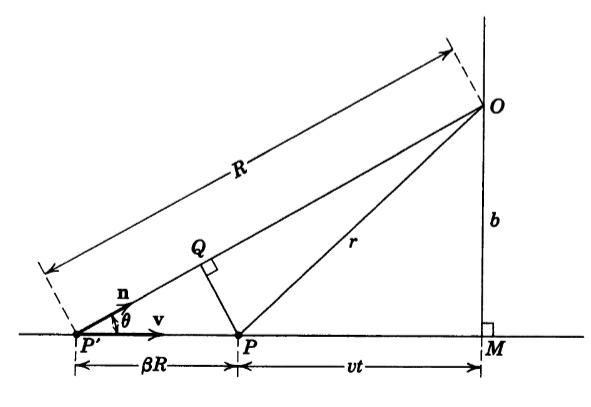
\includegraphics[width=0.6\textwidth]{p2.png} 
\end{center}
Here $O$ is the location of the observer, $P$ is the location of the charged
particle now, $P'$ is the location at the retarded time, and $Q$ is a point on
$OP'$ where a line from $P$ meets $OP'$ at a right angle. $\theta$ is the angle
$OP'$ makes with the $x$ axis. From the setup, it is evident that $PM=vt,OM=b$,
and $OP'=R$ by definition; make sure you understand these assignments.
(Technically since the figure shows the particle on the negative $x$-axis, it is
at $t<0$ and we should write $PM=v\abs{t}$, but $t$ will be squared in the final
result so we can pretend it's positive.)

(a) Use the definition of the retarded time to explain why the segment $P'P$ has
length $\beta R$. Explain geometrically why it then follows that
\begin{equation}
    R(\nhat-\bm\beta)=\vb{r}, 
\end{equation}
where $\vb{r}$ is the vector from the location of the particle \textit{now} to
the observation point (the segment $PO$). This shows that the expression for
$\vb{E}_v$ does indeed point from the location of the particle now.

(b) Show that the lengths of the following segments take the values
\begin{align}
    P'Q&=R\bm\beta\vdot\nhat\notag\\
    OQ&=R(1-\bm\beta\vdot\nhat)\\
    PQ&=\beta b.\notag
\end{align}
For the last equality, use the fact that $\theta$ is in more than one right
triangle.

(c) The segment $PO$ with length $r$ is the hypotenuse of two different right
triangles. Use the Pythagorean theorem for both triangles and equate the values
of $r^2$ to show that
\begin{equation}
    R^2(1-\bm\beta\vdot\nhat)^2=\frac{\tilde{r}^2}{\gamma^2}. 
\end{equation}

(d) Combine the results from part (a) and part (c) to show that the two
expressions for the electric field given above are in fact equal.
\begin{solution}
(a) By definition, the retarded time is
\begin{equation}
    t_\t{ret}=t+\frac{R}{c}, 
\end{equation}
where we have let $-t\to t$ to match the coordinates in the figure. It then
follows that
\begin{equation}
    vt_\t{ret}=vt+\beta R
\end{equation}
is the distance the charge needs to traverse to reach $x=0$, as observed by $O$.
Thus, considering that $vt$ is the distance the charge actually traverse, it
follows that the $PP'$ segment needs to be $\beta R$. By vector addition, we can
then write $R\nhat=\beta R\hat{\bm\beta}+\vb{r}$. Thus,
\begin{equation}\label{p2a:r}
    \vb{r}=R\nhat-R\bm\beta\hat{\bm\beta}=R(\nhat-\bm\beta). 
\end{equation}

(b) First, by Pythagorean theorem, we can write
\begin{equation}
    (PQ)^2=(\beta R)^2-(P'Q)^2=r^2-(R-P'Q)^2
    =r^2-R^2+2R(P'Q)-(P'Q)^2.
\end{equation}
Thus, we can solve for
\begin{equation}
    P'Q=\frac{(1+\beta^2)R^2-r^2}{2R}
    =\frac{(1+\beta^2)R^2-(1+\beta^2-2\bm\beta\vdot\nhat)R^2}{2R}
    =R(\bm\beta\vdot\nhat),
\end{equation}
where we have calculated $r$ from \eqref{p2a:r}. It then follows immediately 
that
\begin{equation}
    OQ=R-P'Q=R(1-\bm\beta\vdot\nhat) .
\end{equation}
Finally,
\begin{equation}
    PQ=\sqrt{\beta^2R^2-(P'Q)^2}
    =R\sqrt{\beta^2-(\bm\beta\vdot\nhat)^2}
    =\beta R\sqrt{1-\cos^2\theta}
    =\beta R\sin\theta
    =\beta R\frac{b}{R}
    =\beta b.
\end{equation}

(c) By the Pythagorean theorem,
\begin{equation}
    r^2=b^2+(vt)^2=(OQ)^2+(PQ)^2
    =R^2(1-\bm\beta\vdot\nhat)^2+\beta^2b^2.
\end{equation}
Thus,
\begin{equation}
    R^2(1-\bm\beta\vdot\nhat)^2=b^2(1-\beta^2)+(vt)^2
    =\frac{\tilde{r}^2}{\gamma^2},
\end{equation}
where $\tilde{r}^2=b^2+\gamma^2(vt)^2$ by definition.

(d) Then, from \eqref{p2:E},
\begin{align}
    \vb{E}=\frac{e\vb{r}}{\gamma^2R^3(1-\bm\beta\vdot\nhat)^3}
    =\frac{e\vb{r}}{\gamma^2\tilde{r}^3/\gamma^3}
    =\frac{\gamma e\vb{r}}{\tilde{r}^3}.
\end{align}
So the two expressions for the electric field are equal.
\end{solution}
\end{problem}
\newpage
%%%%%%%%%%%%%%%%%%%%%%%%%%%%%%%%%%%%%%%%%%%%%%%%%%%%%%%%%%%%%%%%%%%%%%%%%%%%%%%
\end{document}
